% rubber: depend aesfactuur-voorbeeld.tex
\documentclass{article}

\usepackage[dutch]{babel}
\usepackage{url,hyperref,enumitem}
%\usepackage{a4wide}
\usepackage{aes,cursus}

\setlength\parindent{0cm}
\setlength\parskip{1ex}

\setdescription{style=nextline}

\newcommand\meta[1]{\placeholder[#1]}
\newcommand\marg[1]{\cmdarg{\meta{#1}}}

\newcommand\packagenaam{aesfactuur}
\newcommand\packagesf{\textsf{\packagenaam}}

\title{Het \packagesf-package} %\\{\large versie \fileversion}}
\author{\aeskwadraat \TeXniCie\\
\url{hektex@a-eskwadraat.nl}}
%\date{\filedate}

\begin{document}

\maketitle

\section{Introductie}

Met het \packagesf-package kunnen facturen worden gemaakt, in de vorm van een
eenvoudige tabel. In combinatie met de \textsf{aesbrief}-class produceert hij
complete factuurbrieven.

Dit document legt uit hoe je een factuur maakt en hoe de verschillende commando's werken.


\section{Het package laden}

Met \usepack{\packagenaam} bovenaan het document laad je het \packagesf-package.
Er zijn geen opties; alles wordt ingesteld met commando's.

Als je een factuurbrief wilt maken, moet je eerst de \textsf{aesbrief}-class
laden met \class{aesbrief} (met eventule opties).


\section{Factuurinformatie opgeven}

Er zijn allerlei dingen die je kunt instellen. Dat gebeurt door middel
van verschillende commando's die je vrijwel overal tussen \usepack{\packagenaam} 
en \envbegin{factuur} of \envbegin{factuurbrief} kunt plaatsen.

Het commando \cmd{valuta} is altijd beschikbaar:

\begin{description}
\item[\cmd{valuta}\marg{valutasymbool}] Gebruik het opgegeven valutasymbool.
  Standaard is dit \cmd{euro} (\euro). Andere voorbeelden zijn
  \cmd{pounds} (\pounds) en \cmd{\$} (\$).
\end{description}

\subsection{Integratie met de brief}

Wanneer de \packagesf-package wordt ingeladen in een \textsf{aesbrief},
komen daar meer commando's bij:

\begin{description}
\item[\cmd{herinnering}]        Maak van deze factuur een herinneringsfactuur.
\item[\cmd{geenherinnering}]    Maak van deze factuur een normale factuur. Dit is standaard.
\item[\cmd{aanmaning}]			Maak van deze factuur een aanmaning.
\item[\cmd{geenaanmaning}]		Maak van deze factuur een normale factuur.
\item[\cmd{buitenlandbetaling}] Gebruik IBAN- en BIC-informatie%
  \footnote{De benodigde gegevens voor internationaal betalingsverkeer binnen Europa.
            Zie \url{http://nl.wikipedia.org/wiki/International_Bank_Account_Number}
            of de website van je favoriete bank voor meer informatie.}
  bij de betaalinstructie.
\item[\cmd{betalingstermijn}]	Verander de betalingstermijn. Als default wordt 28 dagen gebruikt. Dit commando voor de omgevingsaanroep gebruiken.  
\item[\cmd{binnenlandbetaling}] Gebruik geen IBAN- en BIC-informatie bij de betaalinstructie. Dit is standaard.
\item[\cmd{onsk}\marg{kenmerk}]
  Vergeet deze niet op te geven! Dit commando bestond al in de
  \textsf{aesbrief}-class, maar bij een factuur is het belangrijk om een nummer
  te hebben waar jij, de penningmeester en de ontvanger naar kunnen refereren.
\end{description}

Alle normale commando's voor het instellen van een brief werken hetzelfde als
in een `echte' brief.

Er is ook een stel commando's om allerlei standaardinformatie aan te passen.
Je hoeft ze vrijwel nooit te gebruiken, maar je weet maar nooit:

\begin{description}
\item[\cmd{ovv}\marg{ovv}]   Verander het betaalkenmerk dat de betaler wordt verzocht te vermelden.
\item[\cmd{autoovv}]         Gebruik het met \cmd{onsk} opgegeven kenmerk als betaalkenmerk. Dit is standaard.
\item[\cmd{factuurtitel}\marg{titel}]
  Verander de kop boven de factuur.
\item[\cmd{autofactuurtitel}]
  Bepaal de kop boven de factuur automatisch, aan de hand van de vraag of dit
  een herinneringsfactuur is en of het totaal positief of negatief is.
  Deze optie is de standaard.
\end{description}


\section{De factuur zelf}\label{sec:factuurzelf}

Nu alles is ingesteld, kun je de daadwerkelijke factuur opstellen.

Begin de factuur met \envbegin{factuur} voor een eenvoudige factuur zonder brief.

Als de \textsf{aesbrief}-class is geladen, wil je waarschijnlijk \envbegin{factuurbrief}\marg{adres}
gebruiken. Dit produceert een complete brief met betaalinstructies. Het adres werkt hetzelfde
als bij een normale brief. Let op: in een factuurbrief kun je geen \cmd{opening} gebruiken;
dat is meer iets voor de begeleidende brief.

Nu volgt de factuurinhoud. Die bestaat uit een serie commando's. De volgende zijn beschikbaar:

\begin{description}
\item[\cmd{post}\marg{omschrijving}\marg{bedrag}]
  Voeg een post toe met de gegeven omschrijving.
  Het bedrag wordt neergezet en opgeteld bij het totaal.
\item[\cmd{procent}\marg{omschrijving}\marg{percentage}]
  Voeg een post toe met als bedrag een percentage van het totaal tot nu toe.
\item[\cmd{subtotaal}]
  Voeg een subtotaal-regel in. Het totaal tot nu toe wordt neergezet met een
  mooi kopje en streepje.
\item[\cmd{invul}\marg{omschrijving}]
  Voeg een post toe zonder bedrag; er komen puntjes waarop de ontvanger zelf een
  bedrag moet invullen. \cmd{subtotaal} zal hierna niet meer werken en in plaats
  van het totaal verschijnen er ook puntjes.
\end{description}

Bedragen en percentages bestaan (houd je vast) uit cijfers met mogelijk ergens
een punt of komma, om de scheiding tussen helen en centen aan te geven.
Een minteken voor het bedrag maakt het bedrag of percentage negatief.
Ten slotte: achter een percentage komt geen procentteken.

De factuur wordt be\"eindigd met \envend{factuur} of \envend{factuurbrief}, afhankelijk van
hoe hij begonnen is. Je kunt geen \cmd{closing} gebruiken en er wordt geen ondertekening
neergezet. In plaats daarvan wordt het totaal berekend en volgt een betaalinstructie of,
als het totaal negatief is, een tekst die vertelt dat de ontvanger geld terugkrijgt.


%TODO: meerdere facturen (misschien is meerdere brieven voldoende)
%\section{Meerdere facturen in hetzelfde document}


\section{Voorbeeld}

We sluiten af met een voorbeeld. 
In figuur \ref{fig:code} zie je een voorbeeld-\LaTeX-bestand. De resulterende factuurbrief zie je in figuur \ref{fig:factuur}.

\begin{figure}
\fbox{%
\begin{minipage}{\textwidth}
\verbatiminput{\packagenaam-voorbeeld.tex}
\end{minipage}%
}
\caption{Een voorbeeld van het gebruik van \packagesf.}
\label{fig:code}
\end{figure}

\begin{figure}
\fbox{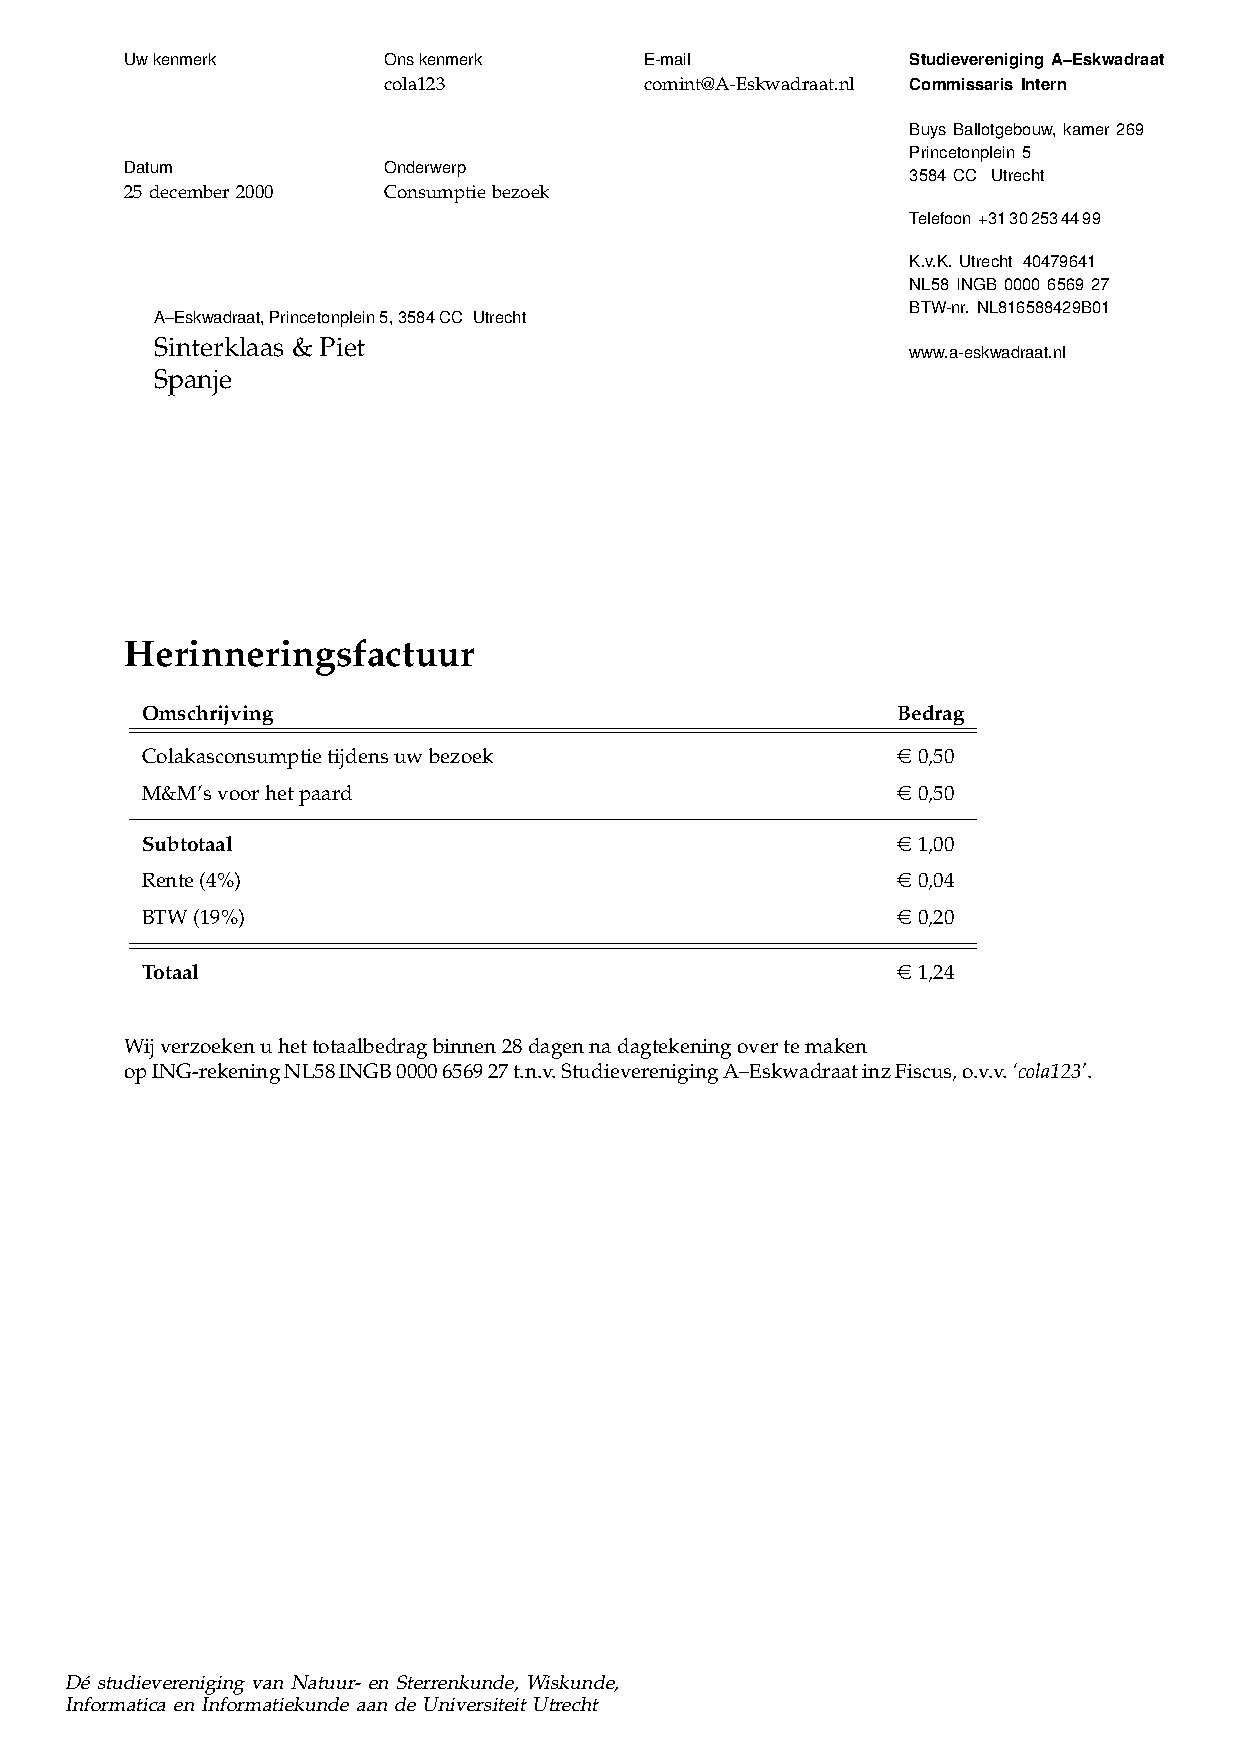
\includegraphics[width=\textwidth]{aesfactuur-voorbeeld}}
\caption{De factuurbrief die het resultaat is van de code in figuur \ref{fig:code}.}
\label{fig:factuur}
\end{figure}

\end{document}
